% No Conserved Program — reversibility and homoiconicity in moop.
% Build (from the repository root):
%   latexmk -pdf -outdir=build/paper -cd docs/paper/paper.tex
%   cp build/paper/paper.pdf docs/paper/paper.pdf
% Figure data and every number in the text come from experiments.c:
%   ./build/experiments docs/paper/data   (see the header of experiments.c)
\documentclass[11pt]{article}

\usepackage[T1]{fontenc}
\usepackage{lmodern}
\usepackage[margin=1in]{geometry}
\usepackage{microtype}
\usepackage{amsmath,amssymb,amsthm}
\usepackage{booktabs}
\usepackage{array}
\usepackage{enumitem}
\usepackage{xcolor}
\usepackage{fancyvrb}
\usepackage{tikz}
\usetikzlibrary{arrows.meta,calc}
\usepackage{pgfplots}
\pgfplotsset{compat=1.18}
\usepackage[numbers,sort&compress]{natbib}
\usepackage[hidelinks]{hyperref}

% Two categorical series: slot 1 and slot 2 of the validated default
% palette (adjacent CVD separation passes); the second series is also
% dashed so identity never rests on hue alone.
\definecolor{moopblue}{HTML}{2A78D6}
\definecolor{harvardorange}{HTML}{EB6834}
\definecolor{inkmuted}{HTML}{52514E}

\newtheorem{theorem}{Theorem}
\newtheorem{lemma}[theorem]{Lemma}
\newtheorem{proposition}[theorem]{Proposition}
\newtheorem{corollary}[theorem]{Corollary}
\newtheorem{observation}[theorem]{Observation}
\theoremstyle{definition}
\newtheorem{definition}[theorem]{Definition}
\theoremstyle{remark}
\newtheorem*{remark}{Remark}

\newcommand{\moop}{\textsf{moop}}
\newcommand{\code}[1]{\texttt{#1}}
\newcommand{\xor}{\oplus}
\newcommand{\lcm}{\operatorname{lcm}}

\title{No Conserved Program:\\[2pt]
  \large Reversibility and Homoiconicity in a Two-Loop Toffoli Machine}
\author{The \moop{} authors\thanks{Draft. Source, harness, and data:
  \code{docs/paper/} in the \moop{} repository.}}
\date{October 2026}

\begin{document}
\maketitle

\begin{abstract}
Reversibility and homoiconicity are usually studied apart: the first as a
property of the semantics and thermodynamics of computation, the second as
a property of how a language represents its own code. We study them
together in \moop{}, a small prototype-based language designed to be
homoiconic throughout, with reversibility reserved for its system-facing
code. Every object's body is two counter-rotating circular tapes coupled
by a pair of Toffoli gates, and user-facing code is kept as data in a
conventional, irreversible layer. We show that this core is exactly a pair of nonlinear feedback
shift registers coupled by one AND term, and we define homoiconicity
structurally, as the absence of an autonomous program subsystem. The
language's own history supplies a control: an early implementation broke
the intended homoiconicity by leaving one tape read-only---a Harvard
machine in miniature---until the wiring was corrected. An exhaustive census
of all $2^{21}$ tape states of the 8/13-cell machine makes the difference
measurable. The control conserves its program and splits into 442,990
orbits, none longer than 255 epochs; the homoiconic wiring has 8,938
orbits, every non-trivial one changes both tapes, and the longest visits
8,191 of the 8,192 possible programs. Across all 100 loop pairs with at
most 22 cells, only 184 short orbits, covering 438 of 78 million states,
restore one tape at every epoch boundary. We then state the synergy
precisely: reversibility makes a state's whole history recoverable, and
homoiconicity makes the program part of that history, so a program that
keeps rewriting itself can still be recovered from any single state.
Because a reversible core never merges states, every many-to-one notion
of ``answer'' must come from a forgetful observation outside it---the
boundary that \moop{}'s two-layer segregation draws. A transcript
theorem, for a calculus of the layer crossings, shows that system
information is lost only by pruning or by exporting it through
observation; and causal pruning, the one internal erasure, provably never
alters the past of the cells it keeps. \moop{} thus occupies two cells of
the reversibility--homoiconicity square on purpose: system-facing code
sits in the causally closed cell, and user-facing code in the homoiconic
but forgetful one, where answers live. Every measured number in the paper is reproduced
by a single harness.
\end{abstract}

%======================================================================
\section{Introduction}
\label{sec:intro}

Two properties of computing systems have been studied by largely
disjoint communities. \emph{Logical reversibility}---every step can be
undone because no step destroys information---comes from the physics of
computation: Landauer's observation that erasure has a thermodynamic
cost~\cite{landauer1961}, Bennett's reversible Turing machines and the
technique of uncomputation~\cite{bennett1973,bennett1989}, and Toffoli and
Fredkin's reversible gates and conservative
logic~\cite{toffoli1980,fredkin1982}. \emph{Homoiconicity}---programs are
data in the same medium the program manipulates---comes from language
design, with Lisp as the canonical example~\cite{mccarthy1960}; its
architectural counterpart is the stored-program idea, in which code lives
in writable memory alongside data~\cite{vonneumann1945}.

Neither literature asks what each property does \emph{for the other}.
The design notes of \moop{}, a small prototype-based language, make a
specific claim about exactly that:
\begin{quote}
\emph{Neither property alone yields any of this: reversibility with an
external program keeps the system irreversible; homoiconicity without
reversibility is self-modification with amnesia.}
\end{quote}
This paper turns that claim into definitions, theorems, and
measurements. The design behind it is specific: \moop{} is meant to be
homoiconic everywhere and reversible only where it faces the system.
Homoiconicity is \emph{layered}---system code is data on the tapes, user
code is data in ordinary memory and, through quotation, a value of the
language---while reversibility belongs to the system-facing code alone. The two properties therefore meet in the
system layer, and the user layer keeps homoiconicity without
reversibility by choice. \moop{}'s objects have reversible bodies built on a single
primitive---two counter-rotating circular tapes (``loops'') coupled by a
pair of Toffoli (CCNOT) gates---and a conventional, forgetful user layer
sits beside them. The core is small enough to enumerate: every state of
the 8/13-cell machine the interpreter uses can be visited.

\paragraph{Contributions.}
\begin{enumerate}[nosep]
\item A closed form for the core: two nonlinear feedback shift registers
  coupled by a single AND term (\S\ref{sec:closed}).
\item A structural definition of homoiconicity---no autonomous program
  subsystem---and an exhaustive orbit census comparing \moop{}'s wiring
  with its own first, Harvard-style wiring
  (\S\ref{sec:homoiconicity}).
\item The synergy as a set of precise statements: recoverable program
  history, no convergence of distinct programs, answers as observations,
  and recurrence (\S\ref{sec:synergy}).
\item Causal pruning, the system layer's one internal erasure, with a
  rewind lemma and an account of what its metadata records
  (\S\ref{sec:pruning}).
\item A transcript theorem for a calculus of the crossings between the
  two layers, showing that every other loss of system information is an
  export through observation (\S\ref{sec:layers}).
\item Consequences for the language surface, including a route to
  general functions as involutions whose forward direction needs only
  user-layer computation (\S\ref{sec:surface}).
\end{enumerate}

\paragraph{Non-claims.} We prove no universality result: the loops are
finite and the wiring is fixed. We describe no hardware and make no
efficiency claim. And \moop{} programs do not execute \emph{on} the
core: the interpreter runs on a conventional host and uses the core for
observation, deposits, and births. Section~\ref{sec:surface} discusses why
this placement is consistent with the theorems.

%======================================================================
\section{Background}
\label{sec:background}

\paragraph{Reversible computing.}
A computation is logically reversible when its step function is
injective, so that the previous state is determined by the current one.
Landauer tied the erasure of a bit to a minimum dissipation of
$kT\ln 2$~\cite{landauer1961}; Bennett showed that any computation can be
made reversible by keeping a history and later uncomputing
it~\cite{bennett1973}, and analysed the space--time cost of doing
so~\cite{bennett1989}. Toffoli's controlled-controlled-NOT gate is
universal for reversible Boolean circuits given constant
ancillae~\cite{toffoli1980}; without ancillae, NOT, CNOT and CCNOT on
$n\ge4$ wires generate exactly the even permutations, and odd ones need a
single extra wire~\cite{shende2003}. Bennett's resolution of Maxwell's
demon locates the unavoidable cost not in measurement, which can be
reversible, but in erasing the demon's memory~\cite{bennett1982}. Toffoli
and Margolus built reversible cellular automata~\cite{toffoli1987}; Morita
surveys reversible machines of many kinds~\cite{morita2017}.

\paragraph{Reversible languages and the place of irreversibility.}
Janus~\cite{lutz1982,yokoyama2007} is a reversible imperative language in
which programs can be inverted syntactically; reversible programs compute
exactly the injective functions~\cite{axelsen2011}. James and Sabry treat
irreversibility as a computational effect over a reversible core, with
the creation and erasure of information as its two
primitives~\cite{james2012}. Causal-consistent
reversibility~\cite{danos2004} tracks dependencies so that concurrent
steps can be undone in a causally consistent order. Knill's QRAM
model~\cite{knill1996} describes a classical host that prepares, drives,
and measures a reversible (unitary) coprocessor. Reversible memory
management has been studied for functional languages~\cite{mogensen2015}.

\paragraph{Two senses of homoiconicity.}
\emph{Representational} homoiconicity means programs are values of the
language's own data structures (Lisp~\cite{mccarthy1960}; reflection in
the sense of Smith~\cite{smith1984}). \emph{Architectural}
homoiconicity is the stored-program concept: code lives in memory that
execution can write. Its opposite is the Harvard organisation, where
the program store is separate and read-only to execution. \moop{} intends both, one per
layer: the architectural kind on the tapes, the representational kind
for user code. Circulating memory as such is old---EDVAC's mercury delay
lines were loops~\cite{vonneumann1945}---so nothing here depends on the
loops being novel.

\paragraph{Shift registers.}
A feedback shift register of length $n$ computes $s_{t+n}=f(s_t,\dots,
s_{t+n-1})$; it is linear (an LFSR) when $f$ is an XOR of taps and
nonlinear (an NLFSR) otherwise~\cite{golomb1967}. Stream ciphers such as
Trivium~\cite{decanniere2008} and Grain~\cite{hell2007} couple shift
registers through AND terms, using state updates that are invertible.

%======================================================================
\section{The machine}
\label{sec:machine}

\begin{definition}[Core]
\label{def:core}
A \emph{core} has two loops, $A\in\{0,1\}^a$ and $B\in\{0,1\}^b$ with
$a,b\ge2$, and two heads $h_A\in\mathbb{Z}_a$, $h_B\in\mathbb{Z}_b$,
initially $0$. One tick is \emph{fire} followed by \emph{rotate}:
\begin{align*}
\textsf{F}:\quad & g \gets A[h_A]\wedge B[h_B];\quad
  A[h_A+1]\gets A[h_A+1]\xor g;\quad B[h_B-1]\gets B[h_B-1]\xor g,\\
\textsf{R}:\quad & h_A\gets h_A+1;\quad h_B\gets h_B-1.
\end{align*}
A tick in which $g=1$ is a \emph{firing}. The \emph{epoch} is
$L=\lcm(a,b)$ ticks, after which both heads are back at their starting
positions. The \emph{epoch map} $E$ sends a tape state $(A,B)$, with
heads at $(0,0)$, to the tape state one epoch later.
\end{definition}

\begin{figure}[t]
\centering
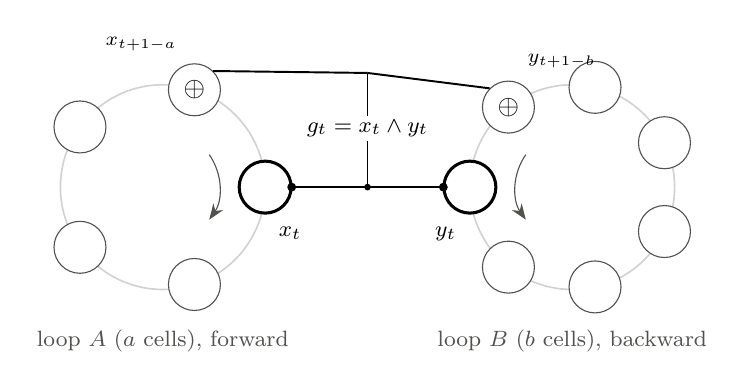
\begin{tikzpicture}[
  cell/.style={circle,draw=inkmuted,fill=white,minimum size=6.6mm,
               inner sep=0pt,font=\footnotesize},
  headcell/.style={cell,draw=black,line width=1.1pt},
  wire/.style={line width=0.7pt},
  lab/.style={font=\footnotesize,text=black},
]
  % the loops themselves
  \draw[gray!35, line width=0.6pt] (0,0) circle (1.3);
  \draw[gray!35, line width=0.6pt] (5.2,0) circle (1.3);
  % loop A: 5 cells, head at 0 deg; the cell at +72 deg arrives next
  \foreach \i in {0,...,4}
    \node[cell] (a\i) at ({72*\i}:1.3) {};
  % loop B: 7 cells around (5.2,0), head at 180 deg; the cell at
  % 180-360/7 deg arrives next (B turns the other way)
  \foreach \i in {0,...,6}
    \node[cell] (b\i) at ($(5.2,0)+({180-360/7*\i}:1.3)$) {};
  \node[headcell] at (a0) {};
  \node[headcell] at (b0) {};
  \node at (a1) {$\xor$};
  \node at (b1) {$\xor$};
  % controls
  \draw[wire] (a0.east) -- (b0.west);
  \fill (a0.east) circle (1.6pt);
  \fill (b0.west) circle (1.6pt);
  % the shared AND drives both targets
  \draw[wire] (2.6,0) -- (2.6,1.45);
  \draw[wire] (2.6,1.45) -- (a1.north east);
  \draw[wire] (2.6,1.45) -- (b1.north west);
  \fill (2.6,0) circle (1.2pt);
  \node[lab,fill=white,inner sep=1.5pt] at (2.6,0.75) {$g_t=x_t\wedge y_t$};
  % labels from Theorem 1
  \node[lab,anchor=north west] at ($(a0.south)+(0.05,-0.05)$) {$x_t$};
  \node[lab,anchor=north east] at ($(b0.south)+(-0.05,-0.05)$) {$y_t$};
  \node[lab,anchor=south east,font=\scriptsize] at ($(a1.north)+(-0.1,0.04)$) {$x_{t+1-a}$};
  \node[lab,anchor=south west,font=\scriptsize] at ($(b1.north)+(0.12,0.04)$) {$y_{t+1-b}$};
  % rotation
  \draw[-{Stealth[length=2mm]},inkmuted] (35:0.72) arc (35:-35:0.72);
  \draw[-{Stealth[length=2mm]},inkmuted] ($(5.2,0)+(145:0.72)$) arc (145:215:0.72);
  \node[lab,text=inkmuted] at (0,-1.95) {loop $A$ ($a$ cells), forward};
  \node[lab,text=inkmuted] at (5.2,-1.95) {loop $B$ ($b$ cells), backward};
\end{tikzpicture}
\caption{One tick of the core. The cells under the heads (thick) are the
controls; their AND $g_t$ is XORed into the next cell of \emph{each}
loop---the cell that rotates under the head next ($\xor$). Labels give
each cell's value in the sequence notation of Theorem~\ref{thm:closed}.
The original wiring had only the target on $A$, so $B$ was never
written.}
\label{fig:machine}
\end{figure}

Figure~\ref{fig:machine} shows one tick. The implementation is 111 lines
of C (\code{src/tapeloop.c}).

\begin{proposition}[Exact inverse]
\label{prop:inverse}
\textsf{F} is an involution and \textsf{R} is a permutation, so a tick
$\textsf{R}\circ\textsf{F}$ is a bijection with inverse
$\textsf{F}\circ\textsf{R}^{-1}$.
\end{proposition}
\begin{proof}
Because $a,b\ge2$, the targets $h_A+1$ and $h_B-1$ are distinct from the
controls $h_A$ and $h_B$, so \textsf{F} does not change $g$. Applying
\textsf{F} twice XORs each target with the same $g$ twice, which is the
identity. \textsf{R} is a rotation of head positions.
\end{proof}

The bound $a,b\ge2$ is necessary. With $a=1$ the target on $A$ is the
control itself. If $B[h_B]=1$, the state with $A=1$ fires and steps to
$A=0$ with $B[h_B-1]$ flipped; the state that already has $A=0$ and
$B[h_B-1]$ flipped does not fire, and steps to the same place. The C function \code{moop\_core\_step\_back} is
$\textsf{F}\circ\textsf{R}^{-1}$---the forward sequence reversed, each
part self-inverse---and a unit test round-trips a full epoch. This shape
returns in \S\ref{sec:surface}.

\paragraph{The control: the original wiring.}
\moop{} was meant to be homoiconic from the start, but the first
implementation of its core (commit \code{2231ab2}) had a single CCNOT,
targeting $A$ only. Loop $B$ was then never written: a read-only program
driving a data loop---a Harvard machine in miniature. That implementation
broke the intent. Commit \code{745ecae} corrected it by adding the
symmetric target on $B$, and in the same change wrote the requirement
down (``no loop may become a read-only program tape''). We keep the
original wiring as a control throughout: the same gate, loops, and
rotation, with and without architectural homoiconicity. We call it the
\emph{Harvard wiring}.

%======================================================================
\section{A closed form: two coupled shift registers}
\label{sec:closed}

Write $A_t,B_t$ for the loops after $t$ ticks, and let
\[
x_t = A_t[t \bmod a],\qquad y_t = B_t[-t \bmod b]
\]
be the cells under the heads at tick $t$. Extend both sequences to
negative indices with the initial tapes: $x_\tau=A_0[\tau\bmod a]$ for
$-a<\tau<0$ and $y_\tau=B_0[-\tau\bmod b]$ for $-b<\tau<0$.

\begin{lemma}[Window]
\label{lem:window}
For all $T\ge0$ and $T-a<\tau\le T$, $A_T[\tau\bmod a]=x_\tau$; likewise
$B_T[-\tau\bmod b]=y_\tau$ for $T-b<\tau\le T$. Each loop holds exactly
the last $a$ (respectively $b$) symbols of its head sequence.
\end{lemma}
\begin{proof}
Cell $i$ of $A$ is under the head at ticks $t\equiv i$ and is a target at
ticks $t\equiv i-1 \pmod a$: it is written only on the tick immediately
before it is read. Let $i=\tau\bmod a$. If $\tau\ge0$, the cell was read
at tick $\tau$ with value $x_\tau$, and its next write happens at tick
$\tau+a-1$, which has not run yet because $\tau+a-1\ge T$. If $\tau<0$,
the cell's first write is at tick $\tau+a-1\ge T$, so it still holds
$A_0[i]=x_\tau$. Loop $B$ is identical with the head moving backward.
\end{proof}

\begin{theorem}[Coupled NLFSRs]
\label{thm:closed}
For all $t\ge0$, with $g_t=x_t\wedge y_t$,
\[
x_{t+1}=x_{t+1-a}\xor g_t,\qquad y_{t+1}=y_{t+1-b}\xor g_t.
\]
\end{theorem}
\begin{proof}
Tick $t$ XORs $g_t$ into $A[(t+1)\bmod a]$, which by
Lemma~\ref{lem:window} (with $T=t$, $\tau=t+1-a$) holds $x_{t+1-a}$; that
cell is the one under the head at tick $t+1$. The same argument applies
to $B$.
\end{proof}

The machine is therefore exactly two shift registers, of lengths $a$ and
$b$, whose feedback shares one nonlinear term. Reversibility is visible
in the recurrence itself, $x_{t+1-a}=x_{t+1}\xor x_ty_t$: the oldest
symbol is recovered from the newer ones. The harness checks the
recurrence, initial conditions included, on 1,000,000 ticks of random
8/13 tapes from $t=0$, with no violations (E1).

\paragraph{The Harvard wiring in closed form.}
With the target on $A$ only, $x$ obeys the same recurrence but
$y_{t+1}=y_{t+1-b}$: loop $B$ is a periodic drive with period $b$, and
$x$ is a register clocked by it. Homoiconicity is, precisely, the shared
term $g_t$ feeding back into \emph{both} registers.

\paragraph{What this explains.}
\moop{}'s primitive observation, MAYBE, steps the core once and returns
the cell under loop $A$'s head: one symbol of the $x$-sequence. It is
``unpredictable-looking but replayable'' for the same reason the
keystream of an invertible NLFSR cipher is. Over $10^6$ draws from
random 8/13 tapes the share of ones is 0.4976 (E7). Births, which seed a
new body from MAYBE draws (\S\ref{sec:layers}), are therefore seeded
from a keystream.

%======================================================================
\section{Homoiconicity as the absence of a conserved program}
\label{sec:homoiconicity}

\begin{definition}[Structural homoiconicity]
\label{def:homoiconic}
A loop is \emph{autonomous} if its next head symbol is a function of its
own past alone. A wiring is \emph{homoiconic} if no loop is autonomous:
every part of the state that acts on the rest is also acted on by it. An
autonomous loop is exactly a ``program tape''.
\end{definition}

By Theorem~\ref{thm:closed}, under \moop{}'s wiring each register's
update depends on the other through $g_t$ (flip $x_t$ while $y_t=1$ and
$y_{t+1}$ flips), so neither loop is autonomous. Under the Harvard wiring
loop $B$ is autonomous. This is the form \moop{}'s intended homoiconicity
takes at the system layer, where there is no instruction encoding on the
tapes; at the user layer it takes the representational form
(\S\ref{sec:surface}).

\begin{proposition}[Harvard conserves its program]
\label{prop:harvard}
Under the Harvard wiring $B$ is invariant, so the state space splits
into $2^b$ sectors, one per program, each closed under the dynamics. No
orbit of the epoch map is longer than $2^a-1$.
\end{proposition}
\begin{proof}
$B$ is never a target. Within a sector the epoch map is a bijection on
the $2^a$ values of $A$, and $A=0$ is fixed because $x\equiv0$ forces
$g\equiv0$.
\end{proof}

\begin{proposition}[Both loops are written]
\label{prop:written}
Under \moop{}'s wiring, every state that is not a fixed point of $E$
fires during its epoch, and every firing flips one cell of each loop.
\end{proposition}
\begin{proof}
If no tick of an epoch fires, the epoch only rotates the heads, which
return; the state is then fixed. A firing XORs $1$ into a target on each
loop.
\end{proof}

Proposition~\ref{prop:written} says neither loop is ever read-only along
a non-trivial orbit. A stronger question is whether a loop can be
written and yet \emph{restored} at every epoch boundary, so that its
epoch-sampled value is conserved along the orbit. That is an empirical
question, and we answer it by enumeration.

\paragraph{Census.}
For nine coprime loop pairs we enumerate every tape state under both
wirings and group the states into orbits of $E$ (E2,
Table~\ref{tab:census}).

\begin{table}[t]
\centering
\small
\begin{tabular}{@{}l l r r r r r r r@{}}
\toprule
loops & wiring & states & orbits & fixed & non-trivial
  & change $A$ & change $B$ & longest \\
\midrule
2/3  & \moop{}  &        32 &       14 &       11 &      3 &      3 &      3 &      11 \\
     & Harvard  &           &       26 &       23 &      3 &      3 &      0 &       3 \\
\addlinespace[2pt]
3/4  & \moop{}  &       128 &       34 &       23 &     11 &     11 &     11 &      31 \\
     & Harvard  &           &       70 &       55 &     15 &     15 &      0 &       7 \\
\addlinespace[2pt]
3/5  & \moop{}  &       256 &       46 &       39 &      7 &      7 &      7 &     109 \\
     & Harvard  &           &      110 &       79 &     31 &     31 &      0 &       7 \\
\addlinespace[2pt]
4/5  & \moop{}  &       512 &       50 &       47 &      3 &      3 &      3 &     233 \\
     & Harvard  &           &      202 &      127 &     75 &     75 &      0 &      15 \\
\addlinespace[2pt]
5/7  & \moop{}  &     4,096 &      194 &      159 &     35 &     35 &     35 &   1,424 \\
     & Harvard  &           &    1,616 &    1,097 &    519 &    519 &      0 &      31 \\
\addlinespace[2pt]
5/8  & \moop{}  &     8,192 &      380 &      287 &     93 &     93 &     93 &   3,053 \\
     & Harvard  &           &    2,552 &    1,631 &    921 &    921 &      0 &      31 \\
\addlinespace[2pt]
7/8  & \moop{}  &    32,768 &      440 &      383 &     57 &     57 &     57 &   9,585 \\
     & Harvard  &           &    5,046 &    4,087 &    959 &    959 &      0 &     127 \\
\addlinespace[2pt]
8/9  & \moop{}  &   131,072 &      850 &      767 &     83 &     83 &     83 &  32,509 \\
     & Harvard  &           &   16,376 &   10,859 &  5,517 &  5,517 &      0 &     255 \\
\addlinespace[2pt]
8/13 & \moop{}  & 2,097,152 &    8,938 &    8,551 &    387 &    387 &    387 & 506,447 \\
     & Harvard  &           &  442,990 &  339,427 & 103,563 & 103,563 & 0 &     255 \\
\bottomrule
\end{tabular}
\caption{Orbits of the epoch map, every tape state enumerated. ``Change
$A$/$B$'' counts the orbits along which that loop's epoch-boundary value
changes; ``longest'' is in epochs. The Harvard bound $2^a-1$
(Proposition~\ref{prop:harvard}) is attained at every size.}
\label{tab:census}
\end{table}

Three things stand out. First, the Harvard wiring never changes $B$, by
construction, and its orbits are short and numerous: at 8/13, 442,990
orbits, none longer than 255 epochs. Second, the homoiconic wiring merges
those sectors into a few long orbits: 8,938 orbits, the longest 506,447
epochs ($\approx52.7$ million ticks), and 99.6\% of states lie on orbits
along which $B$ changes. Third, at these nine sizes \emph{every}
non-trivial orbit changes both loops.

\paragraph{A single orbit tours program-space.}
The longest 8/13 orbit visits 8,191 of the 8,192 possible values of $B$
and 255 of the 256 values of $A$ (E3)---every non-zero ``program'' and
every non-zero ``datum''. Under the Harvard wiring every orbit visits
exactly one program.

\paragraph{Widening the census.}
The nine sizes were chosen before the question was asked, so we swept
every pair $2\le a\le b$ with $a+b\le22$: 100 pairs (54 coprime),
78,293,680 states, and 2,053,629 non-trivial orbits.

\begin{observation}[Restoring orbits are rare and short]
\label{obs:restoring}
In 89 of the 100 pairs, every non-trivial orbit changes both loops'
epoch-boundary values. In the remaining 11 pairs (eight coprime) there
are 184 \emph{restoring} orbits, covering 438 states in total, on which
one loop returns to the same value at every epoch boundary. None is
longer than three epochs. The restored loop is $A$ in seven pairs and $B$
in four (Table~\ref{tab:restoring} in Appendix~\ref{app:sweep}).
\end{observation}

By Proposition~\ref{prop:written}, the restored loop is still written
during every epoch of a restoring orbit. On every restoring orbit the gate
fires between 4 and 16 times per epoch, always an even number
(E2). It must be even: each firing flips one cell of the restored loop,
and a loop comes back only if each of its cells is flipped an even number
of times. So no loop is ever a read-only program tape, but the
orbit-level property is not universal, and we do not claim it is. We have
no characterisation of which sizes admit restoring orbits.

\begin{figure}[t]
\centering
\begin{tikzpicture}
\begin{axis}[
  width=0.92\linewidth, height=6.2cm,
  xmode=log, xmin=1, xmax=1e6,
  ymin=0, ymax=1.03,
  xlabel={orbit length $\ell$ (epochs, log scale)},
  ylabel={share of states on orbits $\le\ell$},
  grid=major, grid style={gray!18},
  axis line style={gray!55}, tick style={gray!55},
  tick label style={font=\small}, label style={font=\small},
  legend style={at={(axis cs:1500,0.8)}, anchor=north west,
                draw=none, font=\small, fill=white},
  legend cell align=left,
]
\addplot[const plot, line width=1pt, color=moopblue]
  table[x=length, y=cumulative] {data/orbits-moop.dat};
\addlegendentry{\moop{} wiring}
\addplot[const plot, line width=1pt, dashed, color=harvardorange]
  table[x=length, y=cumulative] {data/orbits-harvard.dat};
\addlegendentry{Harvard wiring}
\node[font=\footnotesize, anchor=west, text=black]
  at (axis cs:330,0.955) {Harvard: no orbit longer than 255};
\node[font=\footnotesize, anchor=south west, text=black]
  at (axis cs:1.3,0.025) {\moop{}: 0.4\% of states are fixed points};
\end{axis}
\end{tikzpicture}
\caption{Cumulative distribution of the 8/13 tape states by the length
of the orbit they lie on. Under the Harvard wiring every state is on an
orbit of at most 255 epochs; under \moop{}'s wiring most states lie on a
handful of orbits of tens or hundreds of thousands of epochs.}
\label{fig:orbits}
\end{figure}

\paragraph{Reading.}
Dynamically, homoiconicity is the removal of a conservation law: the
program stops being a constant of motion (Figure~\ref{fig:orbits}).
Reversibility then guarantees that removing it costs nothing.

%======================================================================
\section{The synergy, stated precisely}
\label{sec:synergy}

Throughout this section $S$ is a finite state set, $f:S\to S$ is the step
function, and a \emph{program} is a projection $\pi:S\to P$ onto a
designated part of the state. The program trajectory from $s$ is
$P_t=\pi(f^t(s))$. When $f$ is a bijection and all of $S$ is the
machine's state, nothing outside the state is needed to go forward or
back; we call that \emph{causal closure}.

\begin{table}[t]
\centering
\small
\begin{tabular}{@{}l p{0.36\linewidth} p{0.36\linewidth}@{}}
\toprule
 & program conserved (Harvard) & program in mutable state (homoiconic) \\
\midrule
irreversible & data history lost; the program never changes
  & program history can be lost: ``self-modification with amnesia'' \\
reversible & data history recoverable; the program never changes
  & program \emph{and} data history recoverable from any state \\
\bottomrule
\end{tabular}
\caption{The design notes' claim as a $2\times2$. Only the lower-right
cell has a program history that is both non-trivial and recoverable.
\moop{}'s system layer is designed to occupy that cell and its user layer
the upper-right one.}
\label{tab:twobytwo}
\end{table}

\begin{proposition}[The $2\times2$]
\label{prop:twobytwo}
Let $S_0$ be uniformly distributed.
\begin{enumerate}[nosep,label=(\alph*)]
\item If $f$ is a bijection, $H(S_0\mid S_t)=0$ for every $t$; in
  particular the program trajectory $P_0,\dots,P_T$ is a function of any
  single $S_t$.
\item If $f$ merges two states with different programs
  ($f(s)=f(s')$, $\pi(s)\ne\pi(s')$), then $H(P_0\mid S_1)>0$.
\item Under the Harvard wiring $P_t=P_0$ for all $t$.
\item Under \moop{}'s wiring, $P_t=B_t$ is non-constant on every
  non-trivial orbit (Proposition~\ref{prop:written}), and its
  epoch-sampled value is non-constant on all but the restoring orbits of
  Observation~\ref{obs:restoring}.
\end{enumerate}
\end{proposition}
\begin{proof}
(a) $S_0=f^{-t}(S_t)$, and $P_\tau=\pi(f^{\tau-t}(S_t))$. (b) Given
$S_1=f(s)$, which has positive probability, $P_0$ is $\pi(s)$ or
$\pi(s')$, each with positive probability. (c) Proposition~\ref{prop:harvard}.
(d) As stated.
\end{proof}

None of the four parts is deep; their conjunction is the point. Part (b)
says only that a stored-program machine \emph{can} lose program history,
not that it must. Only under both properties is there a program history
that is guaranteed to be both non-trivial (homoiconicity) and recoverable
(reversibility).

\moop{} sits in two cells of Table~\ref{tab:twobytwo} by design. Its
system-facing code, the tapes, is in the lower right: homoiconic and
reversible, hence causally closed. Its user-facing code, the taught
chains of \S\ref{sec:surface}, is in the upper right: homoiconic, and
deliberately forgetful. Corollary~\ref{cor:answers} below says why the
second cell is not a compromise. The Harvard row is the road the
original wiring took by accident.
Table~\ref{tab:twobytwo} summarises.

\begin{proposition}[No convergence]
\label{prop:noconvergence}
If $f$ is a bijection, distinct initial states are never in the same
state at the same time. In a reversible Harvard machine
$f(p,d)=(p,h_p(d))$ with each $h_p$ a bijection on data, if the data
$D_0$ is uniform and independent of the program $P$, then $I(P;D_t)=0$
for all $t$: the data alone says nothing about which program ran.
\end{proposition}
\begin{proof}
The first claim is injectivity of $f^t$. For the second,
$\Pr[D_t=d\mid P=p]=\Pr[D_0=h_p^{-t}(d)]=1/|D|$ for every $p$, so $D_t$ is
uniform and independent of $P$.
\end{proof}

The first part needs only reversibility; it is the
classical-information form of the fact that reversible programs compute
injective functions~\cite{axelsen2011}. The contrast between the wirings
is in the second part. A full state of either machine determines its
program---trivially so under the Harvard wiring, where the program never
changes. But under the Harvard wiring the data never carries any trace
of the program, while under \moop{}'s wiring it does: one epoch from a
uniform 8/13 state, loop $A$ alone carries $I(B_0;A_L)=0.82$ bits about
the initial $B$ ($H(A_L)=8$, $H(A_L\mid B_0)=7.18$), against exactly 0
for the Harvard wiring (E9).

\begin{corollary}[Answers are observations]
\label{cor:answers}
Let a computation's answer be $\mathrm{ans}(s)=\mathrm{obs}(f^T(s))$ for
some observation $\mathrm{obs}:S\to V$. If $f$ is a bijection, then
$\mathrm{ans}(s)=\mathrm{ans}(s')$ for $s\ne s'$ holds only if
$\mathrm{obs}$ identifies the distinct states $f^T(s)\ne f^T(s')$. Every
many-to-one aspect of meaning---two programs with the same answer---is
contributed by the observation, never by the dynamics.
\end{corollary}
\begin{proof}
$f^T$ is injective.
\end{proof}

Corollary~\ref{cor:answers} needs only reversibility, and it constrains
the design rather than dictating it. A reversible core cannot itself
compute an answer in the extensional sense, because it never merges
states: every many-to-one answer must come from a forgetful map outside
it. \moop{}'s segregation realises this constraint. Its bridge shape,
``reversible effect inside, irreversible observation outside''
(\S\ref{sec:layers}), places the forgetful map exactly at the boundary.
Homoiconicity's part is to make the constraint impossible to sidestep. A
Harvard machine can make the identification implicitly, by agreeing to
read only the data; when the program is part of the state there is no
such convention to hide behind, and the forgetting has to be an explicit
observation. The corollary does not say where user programs must run:
Bennett-style compute--copy--uncompute~\cite{bennett1973} runs a whole
computation on a reversible core with only the final copy irreversible.

\begin{proposition}[Recurrence; program identity is the orbit]
\label{prop:recurrence}
If $S$ is finite and $f$ a bijection, every state lies on a cycle, so
every program value $P_t$ recurs. For coprime $a,b$ the tick-level orbits
of a core (tapes and heads) correspond one-to-one with the orbits of $E$,
and each is $L$ times as long.
\end{proposition}
\begin{proof}
A permutation of a finite set decomposes into cycles. For the
correspondence: by the Chinese remainder theorem every head pair is
$(t\bmod a,-t\bmod b)$ for a unique $t\in\mathbb{Z}_L$, so every core
state is reached from a heads-$(0,0)$ state, and a tick-level orbit
passes heads $(0,0)$ exactly at multiples of $L$, where it visits an
orbit of $E$.
\end{proof}

Under homoiconicity, then, every self-modification is eventually undone,
and ``which program is running'' is not well defined; only the orbit is
invariant. The 8/13 machine has exactly 8,938 computations in this sense.
The theorem is about identity, not a mechanism: recurrence can take 52.7
million ticks, and the practical undo is the step-back of
Proposition~\ref{prop:inverse}.

\paragraph{Self-modification with an audit trail.}
The practical face of Proposition~\ref{prop:twobytwo}(a) is time-travel
debugging of code that rewrites itself. The fault may lie in an
instruction that no longer exists, and stepping back recovers it
exactly. Omniscient debuggers~\cite{lewis2003} and record--replay
systems~\cite{ocallahan2017} achieve this by \emph{logging}; for the core
alone the log is unnecessary, because the past is recomputable from the
present. Once the user layer feeds observations back into the core, the
transcript of observations becomes the log
(Theorem~\ref{thm:transcript}).

%======================================================================
\section{Forgetting exactly once: causal pruning}
\label{sec:pruning}

\moop{}'s core has one sanctioned way to lose information. Each cell
carries a mark; a firing marks its two controls and two targets. The
rule records participation in a state change, not counterfactual
dependence: a 0 control that prevented a flip is not marked, although on
a counterfactual account of causation such as Halpern and
Pearl's~\cite{halpern2005} it would count as a cause. \code{moop\_core\_prune} zeroes every unmarked cell, clears the
marks, and starts a new epoch; \code{moop\_core\_run} prunes at every
epoch boundary.

\begin{lemma}[Rewind]
\label{lem:rewind}
Start an epoch at state $S_0$ with clear marks, run $k$ ticks to $S_k$,
and prune to $S'_k$. Running $k$ ticks back from $S'_k$ yields $S_0$ with
the pruned cells zeroed: every kept cell retraces its past exactly.
\end{lemma}
\begin{proof}
Let $U$ be the set of cells unmarked at tick $k$, and let $S'_t$ be $S_t$
with the cells of $U$ zeroed. We show that $S'_t$ steps to $S'_{t+1}$.
If tick $t$ fires in $S_t$, its controls and targets are marked, so they
are not in $U$; $S'_t$ has the same controls and fires on the same
targets. If tick $t$ does not fire in $S_t$, then $S'_t$, whose cells are
pointwise $\le$ those of $S_t$, does not fire either. In both cases the
cells of $U$ are untouched, and they are never targets of a firing in
$S$, so they are constant over $[0,k]$. Hence the trajectories agree off
$U$, and by Proposition~\ref{prop:inverse} stepping back from $S'_k$
retraces $S'_{k-1},\dots,S'_0$.
\end{proof}

The harness confirms the lemma in 100,000 random trials, 41,520 of which
actually prune something, with no mismatches (E5). The lemma is a
statement about the past. It is not the factorisation ``web $\otimes$
inert'' that the design notes once claimed: counterfactually, a 0 cell
that blocked a firing did shape the rest of the state, and a pruned cell
might have fired in a later epoch.

\paragraph{Pruning $\times$ homoiconicity.}
Because code and data share the tapes, an inert cell is dead code and
dead data at once, so garbage collection and dead-code elimination are
one operation. In its extreme form, 8,447 of the $2^{21}$ states of the
8/13 machine never fire during an epoch; at the boundary they are pruned
to zero entirely.

\begin{proposition}[What the marks record]
\label{prop:marks}
Within an epoch, stepping back adds no marks. After $k$ forward ticks from
the start of an epoch, with no steps back, the marks are a function of
$S_k$ and $k$; with epoch-aligned prunes, $k$ is itself a function of the
head positions. After steps back, the marks are those of the furthest
tick reached, which the state does not record.
\end{proposition}
\begin{proof}
Stepping back from $S_{t+1}$ applies $\textsf{R}^{-1}$ and then
\textsf{F} at tick $t$'s alignment. The controls are those of forward
tick $t$, because \textsf{F} never writes its controls, so the back-step
fires if and only if the forward tick did, and marks the same four cells.
For the second claim, rewind $k$ ticks to $S_0$ and replay with clear
marks. For the third, the heads are $(k\bmod a,-k\bmod b)$, which
determine $k$ modulo $L$ by the Chinese remainder theorem (for any $a$
and $b$, coprime or not). The last claim follows from the first.
\end{proof}

The harness confirms the first two claims in 20,000 trials (E6). The
marks are therefore almost, but not quite, a cache. Run forward only,
they are recomputable from the state, and under the project's deletion
test---a construct is redundant if a uniform rule covers all its
uses---pruning would add no state concept of its own. After steps back,
though, they also remember how far the epoch got, which nothing else
records. Two further qualifications apply. Value deposits
(\code{mirrors}, \S\ref{sec:layers}) mark the cells they change, so the
marks also depend on the deposit transcript; birth deposits do not mark,
and exchanges carry marks with their bits. And stepping back \emph{past}
the start of an epoch marks cells from the previous epoch's firings.

\paragraph{Where pruning matters.}
Pruning is a sparsity phenomenon. Table~\ref{tab:density} and
Figure~\ref{fig:density} show the share of initially set bits that are
still inert after the first epoch of random 8/13 tapes (E4). At 2\%
density 82.9\% of set bits are pruned; at 50\% density, 0.2\%.

\begin{table}[t]
\centering
\small
\begin{tabular}{@{}l r r r r r r r r r@{}}
\toprule
density & 2\% & 4\% & 6\% & 8\% & 10\% & 20\% & 30\% & 40\% & 50\% \\
\midrule
set bits pruned & 82.9 & 68.4 & 55.5 & 44.6 & 35.7 & 12.0 & 3.4 & 0.9 & 0.2 \\
runs that prune & 30.9 & 46.1 & 51.9 & 50.0 & 45.5 & 19.7 & 6.2 & 1.5 & 0.3 \\
\bottomrule
\end{tabular}
\caption{First-epoch pruning on random 8/13 tapes, 4,000 runs per
density (percentages). Fewer runs prune at 2\% than at 6\% because very
sparse tapes often start with nothing set at all.}
\label{tab:density}
\end{table}

\begin{figure}[t]
\centering
\begin{tikzpicture}
\begin{axis}[
  width=0.8\linewidth, height=5.4cm,
  xmin=0, xmax=52, ymin=0, ymax=100,
  xlabel={density of set cells (\%)},
  ylabel={set bits pruned (\%)},
  grid=major, grid style={gray!18},
  axis line style={gray!55}, tick style={gray!55},
  tick label style={font=\small}, label style={font=\small},
]
\addplot[color=moopblue, line width=1pt, mark=*, mark size=1.7pt,
         mark options={fill=moopblue, draw=white, line width=0.4pt}]
  table[x=density, y=inert] {data/pruning.dat};
\end{axis}
\end{tikzpicture}
\caption{Share of initially set bits pruned at the first epoch boundary,
by tape density (8/13 cells, 4,000 runs per point).}
\label{fig:density}
\end{figure}

\paragraph{Landauer accounting.}
The prune's return value counts the set bits it clears, and it destroys
at most as many bits of information as there are unmarked cells. That
budget is the system layer's \emph{entire} internal erasure---the
analogue, in this design, of the checkpoints at which a Bennett-style
computation discards its history~\cite{bennett1989}.

\paragraph{The running language does not prune.}
The interpreter steps bodies through MAYBE and never calls
\code{moop\_core\_run}, so no \moop{} program prunes today. Turning it on
would not be a one-line change. A birth draws $a+b$ ticks from its
generator, and a prune inside that window would break the generator's
ability to rewind to before the birth (\S\ref{sec:layers}). When a body
may prune without breaking the promises made by births is an open
question.

%======================================================================
\section{Two memories, two logics}
\label{sec:layers}

\moop{} segregates its machine into two layers (Table~\ref{tab:layers}).
Corollary~\ref{cor:answers} says why answers need a forgetful layer. This section
makes precise what may cross between them.

\begin{table}[t]
\centering
\small
\begin{tabular}{@{}l l l@{}}
\toprule
 & system layer & user layer \\
\midrule
memory & the tape loops of every body & conventional, overwritable memory \\
operators & NOT, CNOT, CCNOT, SWAP (self-inverse) & AND, OR, NAND, NOR, XOR, MAYBE \\
character & never loses information (except pruning) & forgets freely \\
\bottomrule
\end{tabular}
\caption{The two layers.}
\label{tab:layers}
\end{table}

\paragraph{Placement by information behaviour.}
XOR appears on both sides. As a two-input, one-output function it
discards an input and belongs to the user layer; as CNOT it computes the
same XOR in place, keeps its control, and belongs to the gate layer. What
places an operator is whether its inputs survive, not which Boolean
function it computes.

\paragraph{A calculus of crossings.}
Let $\sigma\in\Sigma$ be the system state (all tapes and heads) and
$\rho\in R$ the user state. A \emph{program} is a fixed sequence of
instructions of five kinds:
\begin{itemize}[nosep]
\item $\mathsf{sys}(g)$: $\sigma\gets g(\sigma)$, with $g$ a bijection of
  $\Sigma$ (a step, a step-back, or an exchange of two bodies' tapes);
\item $\mathsf{obs}(\pi,u)$: emit $o=\pi(\sigma)$ to the
  \emph{transcript}, then $\rho\gets u(\rho,o)$;
\item $\mathsf{dep}(q,\{g_v\})$: $\sigma\gets g_{q(\rho)}(\sigma)$, where
  every $g_v$ is a bijection of $\Sigma$ (an XOR deposit of the value
  $v$);
\item $\mathsf{usr}(h)$: $\rho\gets h(\rho)$, with $h$ arbitrary;
\item $\mathsf{new}(n)$: append $n$ blank cells to $\sigma$.
\end{itemize}
MAYBE is $\mathsf{sys}(\text{step})$ followed by $\mathsf{obs}$ of the
head cell; the innate \code{value} message is $\mathsf{obs}$ of loop $A$;
\code{n mirrors box} is $\mathsf{dep}$.

\begin{theorem}[Transcript]
\label{thm:transcript}
Run a prune-free program from $(\sigma_0,\rho_0)$ to
$(\sigma_T,\rho_T)$, producing transcript $O$.
\begin{enumerate}[nosep,label=(\roman*)]
\item $\rho_T$ is a function of $\rho_0$ and $O$: the user layer sees the
  system only through the transcript.
\item $\sigma_0$ is a function of $\sigma_T$, $\rho_0$, and $O$.
\item If no deposit's value depends on $O$ (open loop), then
  $\sigma_0\mapsto\sigma_T$ is injective for each fixed $\rho_0$.
\end{enumerate}
\end{theorem}
\begin{proof}
(i) By induction: only $\mathsf{obs}$ and $\mathsf{usr}$ change $\rho$,
and they use only $\rho$ and the emitted $o$. (ii) By (i), replaying the
user layer from $\rho_0$ and $O$ yields every deposit value $v_i$. Now
invert the system half in reverse order: $\mathsf{sys}(g)$ by $g^{-1}$,
$\mathsf{dep}$ by $g_{v_i}^{-1}$, and $\mathsf{new}$ by dropping the
appended cells, while $\mathsf{obs}$ and $\mathsf{usr}$ leave $\sigma$
alone. (iii) The inverse in (ii) then uses no part of $O$.
\end{proof}

Part (iii)'s hypothesis cannot be dropped. Observing a body's value and
depositing it back (a fresh session),
\begin{Verbatim}[fontsize=\small,xleftmargin=2em]
moop> box is a world
moop> box ask value
181
moop> n is box ask value
moop> n mirrors box
a proto
moop> box ask value
0
moop> n mirrors box
a proto
moop> box ask value
181
\end{Verbatim}
blanks the body's loop $A$, because $A\xor A=0$, and depositing
\code{n} again restores it. (A \code{mirrors} answers with the body it
changed, which the REPL prints as \code{a proto}.) On the 8/13 tapes this
closed loop maps all $2^{21}$ states onto 8,192 (E8). Nothing has been
lost yet: \code{n} still holds the value. The loss happens only when the
user layer forgets \code{n}. This is reset by measurement and feedback, and it is exactly
Bennett's account of Maxwell's demon~\cite{bennett1982}: the measurement
is reversible, and the cost is paid when the demon's memory is erased.
Here the user layer is the demon's memory.

\begin{corollary}[Erasure is pruning or export]
\label{cor:export}
In the calculus extended with pruning---and in \moop{}, to the extent
that its C code follows the calculus (\S\ref{sec:limits})---the system
layer destroys information without a record only by pruning. Every other
loss is an export through observation: given the user layer's initial
state, it is recorded in the transcript, and it becomes physical erasure
only when the user layer forgets.
\end{corollary}

The harness checks Theorem~\ref{thm:transcript}(ii) on 100,000 random
closed-loop programs of 64 instructions each (2,560,676 observations):
the initial tapes were recovered every time (E8). The unit tests include
the same check and the REPL reset above.

\paragraph{The crossings.}
Table~\ref{tab:crossings} maps every crossing onto the vocabulary of
\S\ref{sec:background}. The system layer is information-preserving
except at these four points. Births are not a fifth: since the changes
described in this paper, a birth is literally \textsf{new}, then one
MAYBE draw per cell from the generator, each deposited onto a blank
cell with CNOT. The C code asserts that the child's cells are blank.

\begin{table}[t]
\centering
\small
\begin{tabular}{@{}l l l@{}}
\toprule
crossing & \moop{} construct & known as \\
\midrule
copy out & \code{maybe}, \code{value} (observation) & measurement (QRAM~\cite{knill1996}) \\
controlled in & \code{n mirrors box} (XOR deposit) & classically controlled gate \\
create & blank cells for a birth & \emph{create}~\cite{james2012}; ancilla \\
erase & epoch prune & \emph{erase}~\cite{james2012}; Landauer \\
\bottomrule
\end{tabular}
\caption{Every point at which information crosses into or out of the
system layer. A birth is \emph{create}, then copy out, then controlled
in.}
\label{tab:crossings}
\end{table}

In linear-logic terms~\cite{girard1987} the core is linear: no step
duplicates or discards. A birth is a controlled \emph{contraction}
(fresh cells receive copies of observations) and pruning a controlled
\emph{weakening}, the ``discharge of premises that were never used in any
inference'' in the project's own phrase.

\paragraph{Actors and protos.}
\moop{}'s objects sit on this boundary. An actor's body is a core and
its surface is a table of hosted, irreversible messages. Undo the
body's reversible steps and its whole state returns; the replies it
gave are the only irreversible product. The irreversibility lives
entirely in what was \emph{said}, never in what \emph{is}. Protos add
two relations that \moop{} keeps apart. \emph{Generation} (who made
you) is the only downward path from system to user layer, and it costs
the generator nothing irreversible: step it back $a+b$ ticks and it
returns to the moment before the birth. \emph{Delegation} (whom you
defer to) walks parent links that are fixed at birth, among user-facing
protos only, and never crosses the boundary.

%======================================================================
\section{The synergy at the language surface}
\label{sec:surface}

\moop{} has one grammar rule and four relational operators whose arrow
shapes follow information behaviour: \code{ask}~(\code{->}) sends a
message and \code{inherits}~(\code{<-}) tests lineage, both one-way and
forgetful; \code{mirrors}~(\code{<->}) is two-way and gate-backed;
\code{is} names. The indefinite article births: \code{rex is a dog}
introduces a new proto generated from \code{dog}, while \code{rex is
dog} only aliases it. The syntax follows Quorum's evidence that words
read better than symbols for novices~\cite{stefik2013}, and the object
model follows Self and Io~\cite{ungar1987,dekorte2005} in using
prototypes rather than classes.

\paragraph{Code that is its own inverse.}
Every \code{mirrors} form is an involution: \code{5 mirrors box}
XOR-deposits 5 onto the body's loop $A$, and \code{box mirrors other}
swaps two bodies' $A$-loops. Applying either twice is the identity
(tested), so for these forms the program text is its own undo.

\paragraph{General functions, without a new form.}
The design notes list number-to-number bijections under \code{mirrors}
(``\code{celsius mirrors fahrenheit}'') as open. The analysis above
reduces half of that problem. The standard reversible
embedding~\cite{toffoli1980,bennett1973} turns any function $f$,
reversible or not, into the involution $(x,y)\mapsto(x,y\xor f(x))$, and
\moop{}'s deposit already accepts any number on its left. With $f$ the
identity it works today, in a fresh session:
\begin{Verbatim}[fontsize=\small,xleftmargin=2em]
moop> c is a world
moop> f is a world
moop> c ask value
181
moop> f ask value
52
moop> c ask value mirrors f
a proto
moop> f ask value
129
moop> c ask value mirrors f
a proto
moop> f ask value
52
\end{Verbatim}
This is a CNOT copy between bodies ($52\xor181=129$), and doing it twice
is the identity. For the forward direction, then, no new \code{mirrors}
form is needed; what is missing is a way to compute $f$ in the user
layer---arithmetic or logic operators, and messages that take
arguments. The embedding never computes $f^{-1}$, though, which a
two-way reading of \code{celsius mirrors fahrenheit} implies, and
\code{1 mirrors 2} is still refused. So the deletion test does not
dissolve the whole construct. In-place bijections are the other route: a
bijection written as a sequence of involutions is inverted by reversing
the sequence---exactly the shape of $\textsf{F}\circ\textsf{R}^{-1}$ in
Proposition~\ref{prop:inverse}. NOT, CNOT and CCNOT build every even
permutation of $n$-bit values ($n\ge4$), and every permutation with one
extra bit~\cite{shende2003}. Reversing a
chain is an operation on code as data. \moop{}'s reflection (below)
makes code a value, but not yet one that can be taken apart, so this
route still needs structural editing of code.

\paragraph{Layered homoiconicity: reversible where system-facing.}
\moop{}'s user code is homoiconic in its own medium: a taught message
body is the parser's chain structure, stored and run at each send.
Re-teaching a message \emph{replaces} the chain---homoiconicity without
reversibility, the upper-right cell of Table~\ref{tab:twobytwo}. That is
the design, not a gap: \moop{} reserves reversibility for system-facing
code, and by Corollary~\ref{cor:answers} the user layer is where answers
live, and answers require forgetting. The causal closure of
\S\ref{sec:synergy} therefore holds exactly where it was meant to, in
system-facing code. Keeping user
programs in the irreversible layer, off the tapes, is consistent with the
same corollary but not required by it, since compute--copy--uncompute
could run them on a reversible core. The project's rule that nothing
user-facing goes on the tapes is a design choice the theorems permit,
not one they force.

\paragraph{Reflection: quotes mention code.}
User-layer homoiconicity is reached through the oldest device written
English has for the distinction between using words and mentioning them:
quotation marks. A quote is the quoted statement itself, as a value,
parsed but never evaluated; quotes nest by alternating double and single
marks, as in English prose. In message position a quoted name is
mentioned rather than sent, so it designates the receiver's code for
that message, found by the same lookup a send uses. With \code{is} it
designates the place where that code lives:
\begin{Verbatim}[fontsize=\small,xleftmargin=2em]
moop> dog is a world
moop> dog ask mood is ask maybe
moop> dog ask "mood"
"ask maybe"
moop> cat is a world
moop> cat ask "mood" is dog ask "mood"
moop> cat ask "mood"
"ask maybe"
\end{Verbatim}
The quote moves across \code{is}: \code{x ask m is c} and
\code{x ask "m" is "c"} teach the same thing, so teaching needed no new
form. Running a code value needed none either---teach it, then ask---so
by the deletion test there is no \code{eval}. Reads and writes copy, so
a code value never aliases a teaching. Code prints back in canonical
spelling, which can be typed in again. What reflection does not yet
provide is structural editing: code can be named, read, copied, and
installed, but not taken apart or assembled from pieces. That waits for
user-layer data operators and message arguments, which \moop{} does not
have for any kind of data yet.

%======================================================================
\section{Method and reproducibility}
\label{sec:method}

All experiments are in one C file, \code{docs/paper/experiments.c},
linked against the real core; the Harvard control reimplements the
original \code{fire} function. E2, E3, E9 and the sweep are
exhaustive and therefore exact. E1 (50 runs of 20,000 ticks, checked
from $t=0$ with the initial conditions of Theorem~\ref{thm:closed}), E4 (4,000 runs per
density), E5 (100,000 trials), E6 (20,000), E7 ($10^6$ draws), and E8
(100,000 programs) use a fixed-seed xorshift generator, so every number
reproduces. (The REPL transcripts come from the interpreter and the line
count from the source.) The whole harness runs in about a minute and a
half on one
core and writes the data behind Figures~\ref{fig:orbits}
and~\ref{fig:density}. The repository's unit tests (\code{make test})
cover the invariants the paper relies on: the round-trip, both loops
transformed, the 4/5 orbit census, involutions, the rewind lemma, the
marks within an epoch, the transcript recovery, the gate-backed births,
and the generator's rewind.

%======================================================================
\section{Limitations and threats to validity}
\label{sec:limits}

\begin{enumerate}[nosep]
\item \textbf{The language does not execute on the core.} The core is a
  substrate for objects' bodies, not the processor that runs the
  program. Section~\ref{sec:surface} argues this placement is consistent with
  Corollary~\ref{cor:answers}, but it means \moop{} is not a
  non-von-Neumann \emph{computer}; it is a language whose objects have
  reversible bodies.
\item \textbf{No universality.} The loops are finite and the wiring is
  fixed; the project's phrase ``Turing tape'' is a misnomer for
  fixed-length loops. A universality result would need unbounded loops
  and an embedding of a known universal reversible system.
\item \textbf{Structural, not instruction-level, homoiconicity.} There
  is no instruction encoding on the tapes, so our results concern state,
  not code in the usual sense. At the user layer, code is a value
  (reflection by quotation) but cannot yet be taken apart or built from
  pieces.
\item \textbf{The orbit-level property is not universal.} Observation~%
  \ref{obs:restoring} is exhaustive only up to $a+b\le22$, for one wiring,
  and it has exceptions; we have no characterisation of them.
\item \textbf{Recurrence is conceptual.} Recurrence times of tens of
  millions of ticks make Proposition~\ref{prop:recurrence} a statement
  about identity, not an undo mechanism.
\item \textbf{Pruning is barely exercised.} It rarely acts on dense
  tapes (Table~\ref{tab:density}), the running language never prunes,
  and a manual mid-epoch prune breaks the recovery of the tick count from
  the heads.
\item \textbf{The user layer is partly nominal.} The interpreter keeps
  user state in ordinary C structures rather than the RAM module, and
  of the user logic only MAYBE is reachable from the surface.
\item \textbf{Segregation is enforced by convention.} The C modules
  respect the layer rules by discipline; Theorem~\ref{thm:transcript}
  holds for the calculus, not for arbitrary C. A type or effect system
  would enforce it.
\end{enumerate}

%======================================================================
\section{Related work}
\label{sec:related}

\paragraph{Reversible computing.}
\moop{}'s core is a reversible dynamical system in the tradition of
conservative logic and reversible cellular
automata~\cite{fredkin1982,toffoli1987,morita2017}. Its distinguishing
choices are a single gate pair on two counter-rotating loops and the
requirement that no loop act as a program. Bennett's analysis of
uncomputation~\cite{bennett1973,bennett1989} is the model for treating
pruning as the one, explicit discard. Reversible processors such as
Pendulum~\cite{vieri1999} target hardware efficiency; we make no
efficiency claim.

\paragraph{Reversible languages.}
Janus~\cite{lutz1982,yokoyama2007} and its successors make whole
programs reversible and invert them syntactically. \moop{} instead keeps
a reversible substrate under an irreversible surface. The closest work is
James and Sabry's information effects~\cite{james2012}, which treat
creation and erasure of information as effects layered on a reversible
core. \moop{}'s crossings map onto theirs (Table~\ref{tab:crossings}),
adding observation and classically controlled deposits from the QRAM
model~\cite{knill1996}. Our transcript theorem has the flavour of their
results for an untyped, object-based setting. Reversible garbage
collection~\cite{mogensen2015} and causal-consistent
reversibility~\cite{danos2004} are related to pruning and its causal
marks.

\paragraph{Homoiconicity and reflection.}
Lisp~\cite{mccarthy1960} and reflective towers~\cite{smith1984} are
representationally homoiconic, and so is \moop{}'s user layer, with
quotation in place of Lisp's \code{quote} and no \code{eval}. Our
structural definition for the system layer is closer to the
stored-program concept~\cite{vonneumann1945}, phrased dynamically: no
autonomous program subsystem.

\paragraph{Shift registers.}
Theorem~\ref{thm:closed} places the core among coupled NLFSRs, the state
machines of hardware-oriented stream ciphers~\cite{decanniere2008,
hell2007,golomb1967}. We use the connection only to explain the
behaviour of MAYBE and make no cryptographic claim.

\paragraph{Objects, actors, and syntax.}
Self~\cite{ungar1987} and Io~\cite{dekorte2005} are prototype-based;
actors~\cite{hewitt1973} inspired \moop{}'s non-hereditary actors; and
Quorum's empirical work on syntax~\cite{stefik2013} motivates its word
operators.

\paragraph{Debugging.}
Omniscient debugging~\cite{lewis2003} and record--replay~\cite{
ocallahan2017} provide backward execution by logging; causal closure
provides it by recomputation.

%======================================================================
\section{Future work}
\label{sec:future}

The most direct next steps are:
\begin{itemize}[nosep]
\item characterise the loop sizes that admit restoring orbits, and prove
  Observation~\ref{obs:restoring} where it holds;
\item expose user-layer computation (logic words, arguments), so that
  the Bennett-embedding route to general functions becomes usable;
\item settle how pruning and generation share a body, then let the
  running language prune;
\item enforce the segregation with a type or effect system that has
  Theorem~\ref{thm:transcript} as a soundness result;
\item add structural editing of code values, enabling inversion by
  reversal;
\item look for universality with unbounded loops or a ring of gates;
\item reclaim pruned cells (shrinking the loops) rather than zeroing
  them in place.
\end{itemize}

%======================================================================
\section{Conclusion}
\label{sec:conclusion}

Homoiconicity removes the conserved program; reversibility makes the
removal lossless. A machine with both properties remembers every
program it has been; because it never lets two states converge, it
cannot itself say that two computations meant the same thing---only an
observation can. \moop{}'s two memories put that observation at the
boundary: homoiconic everywhere, reversible where it faces the system,
and forgetful only where answers are made. Its one internal
act of forgetting, causal pruning, removes only what never decided
anything, and every other loss is an export that the user layer, like
Maxwell's demon, pays for when it forgets.

\bibliographystyle{plainnat}
\bibliography{refs}

\appendix

%======================================================================
\section{Restoring orbits in the sweep}
\label{app:sweep}

\begin{table}[h]
\centering
\small
\begin{tabular}{@{}l r r r r r@{}}
\toprule
loops & non-trivial orbits & restore $A$ & restore $B$ & states on them
  & longest (epochs) \\
\midrule
5/6        &    45 &  0 &  3 &   6 & 2 \\
2/13       &   257 &  2 &  0 &   6 & 3 \\
5/11       &   175 &  0 & 11 &  22 & 2 \\
2/15       &   689 &  8 &  0 &  24 & 3 \\
5/13       &   225 &  0 &  5 &  10 & 2 \\
8/10$^*$   & 1,457 &  6 &  0 &  12 & 2 \\
2/17       & 1,601 & 20 &  0 &  60 & 3 \\
6/14$^*$   & 2,332 &  8 &  0 &  16 & 2 \\
2/19       & 3,915 & 40 &  0 & 120 & 3 \\
5/16       &   483 &  0 & 24 &  48 & 2 \\
10/12$^*$  & 4,773 & 57 &  0 & 114 & 2 \\
\bottomrule
\end{tabular}
\caption{The 11 of 100 loop pairs ($2\le a\le b$, $a+b\le22$) that have
restoring orbits under \moop{}'s wiring ($^*$: lengths not coprime).
Totals: 184 orbits on 438 of 78,293,680 states.}
\label{tab:restoring}
\end{table}

%======================================================================
\section{A REPL session}
\label{app:repl}

Births, teaching, delegation, the lineage predicate, and \code{mirrors}
applied twice:
\begin{Verbatim}[fontsize=\small,xleftmargin=2em]
moop> animal is a world
moop> animal ask mood is
....>     ask maybe
....>
moop> cat is an animal
moop> cat ask mood is 9
moop> dog is an animal
moop> dog ask mood
false
moop> cat ask mood
9
moop> dog inherits animal
true
moop> box is a world
moop> box ask value
52
moop> 5 mirrors box
a proto
moop> box ask value
49
moop> 5 mirrors box
a proto
moop> box ask value
52
\end{Verbatim}

%======================================================================
\section{The design history as a derivation chain}
\label{app:history}

\moop{}'s commit messages narrate its history as a sequence of
derivations, each change justified by an axiom, with some constructs
later derived away. The table lists the rationale each commit records.
Homoiconicity was intended from the start; it was first written down in
the same commit that corrected the wiring.

\begin{table}[h]
\centering
\small
\begin{tabular}{@{}l p{0.38\linewidth} p{0.4\linewidth}@{}}
\toprule
commit & change & rationale recorded \\
\midrule
\code{2231ab2} & one CCNOT on two counter-rotating loops & reversibility: gate plus permutation \\
\code{53954f3} & two memories, two logics & segregation of reversible and irreversible operators \\
\code{7290131} & causal pruning & one explicit, sanctioned erasure \\
\code{745ecae} & symmetric targets on both loops & homoiconicity: no read-only program tape \\
\code{6a23e49} & non-hereditary actors & the bridge shape, generalised to objects \\
\code{a9405bf} & protos: generation apart from delegation & orthogonality of who-made-you and whom-you-defer-to \\
\code{e2309ff} & \code{<->} as involutions & bijective as a tested fact \\
\code{843353e} & \code{self} removed (headless chains) & deletion test: every context has a receiver \\
\code{5c17b4c} & \code{generate} removed (the article) & deletion test: introduction instantiates \\
\code{0dd9521} & births as create + observe + deposit & the bridge shape; deletion test on birth as a crossing \\
\code{4ca5af7} & reflection: quotes mention code & ubiquitous homoiconicity; deletion test removes \code{eval} \\
\bottomrule
\end{tabular}
\caption{Selected commits and the rationale each records.}
\label{tab:history}
\end{table}

\end{document}
